\documentclass{article}
\usepackage[T1]{fontenc}
\usepackage[utf8x]{inputenc}
\usepackage[polish]{babel}
\usepackage{graphicx}
\usepackage[export]{adjustbox}
\usepackage{amsmath}
\usepackage{hyperref}
\hypersetup{
	colorlinks,
	linktoc = all,
	linkcolor = black
}
\usepackage{subcaption}
\usepackage{wrapfig}


\title
{
	Projektowanie i analiza algorytmów \\
	Sprawozdanie \\
	Miniprojekt 1
}
\author{Filip Juchnowicz \vspace{10pt}\\ Indeks 264176}
\date{03.04.2023}

% 1
% 2
% [3]
% [4]
% 5
% [8]
% [9]

\begin{document}
	
	\maketitle
	\thispagestyle{empty}
	
	\newpage
	
	\tableofcontents
	\listoffigures
	
	\newpage
	
	\section{Zadanie 1 - Tablice dynamiczne.}
	Tablica jest tworzona poprzez przypisanie zmiennej jednego ciągu adresów w pamięci o podanym rozmiarze (np. 2x4 - 8 komórek). 
	\subsection{Operacje na tablicy.}
	\subsubsection{Wypełnianie tablicy losowymi wartościami}
	Funkcja odwołuje się do tablicy poprzez wskaźnik. Ponieważ tablica jest jednym dużym blokiem adresów odwołanie polega na wskazanie wiersza ($i*n$), a następnie kolumny ($+j$).
	\begin{figure}[h]
		\centering
		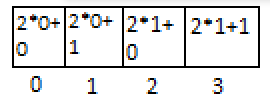
\includegraphics[width=0.4\linewidth]{pics/fill_array_ex}
	\end{figure}
	
	\begin{itemize}
		\item Złożoność obliczeniowa: O($nm$),
		\item Złożoność pamięciowa: O(1).
	\end{itemize}
		\begin{figure}[h]
		\centering
		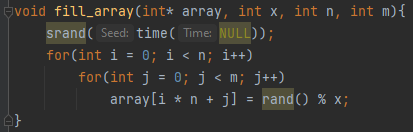
\includegraphics[width=0.6\linewidth]{pics/fill_array.png}
			\caption{Funkcja wypełniająca tablice wartościami z zakresu <0; x>}
		\end{figure}
	
	\subsubsection{Wyświetlanie tablicy}
	Wyświetlanie działa identycznie jak wypełnianie wartościami.
	\begin{figure}[h]
		\centering
		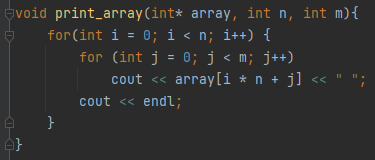
\includegraphics[width=0.6\linewidth]{pics/print_2d_array}
		\caption{Funkcja wyświetlające zawartość tablicy w terminalu.}
	\end{figure}
	
	\newpage
	\subsubsection{Znajdź maksymalny element}
	Funkcja jest kolejną modyfikacją funkcji wypełniającej tablice. Zawiera dodatkową zmienną (szukane max) oraz warunek sprawdzający czy aktualny element jest większy od zapisanego max.
	\begin{figure}[h]
		\centering
		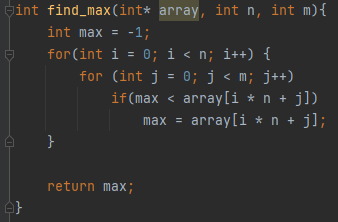
\includegraphics[width=0.6\linewidth]{pics/array_findmax}
		\caption{Funkcja znajdująca maksymalny element w tablicy.}
	\end{figure}
	
	
	\subsection{Zapis tablicy do pliku}
	\subsubsection{tekstowego}
	Funkcje działają podobnie jak poprzednie. Liczby są pojedynczo wpisywane/sczytywane uwzględniając znak nowej linii na końcu.
	\begin{figure}[h]
		\centering
		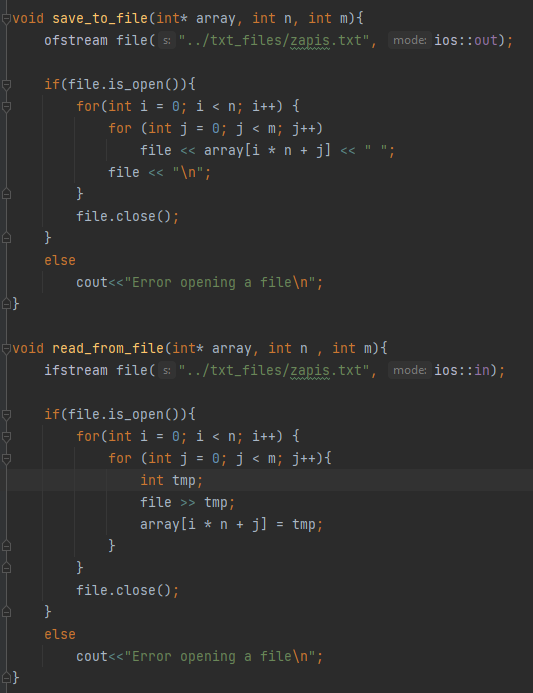
\includegraphics[width=0.45\linewidth]{pics/array_file}
		\caption{Zapis tablicy do pliku tekstowego.}
	\end{figure}
	
	
	\subsubsection{binarnego}
	Zapisywanie do pliku binarnego polega na wpisaniu danych na zadeklarowany blok o odpowiednim rozmiarze.
	\begin{figure}[h]
		\centering
		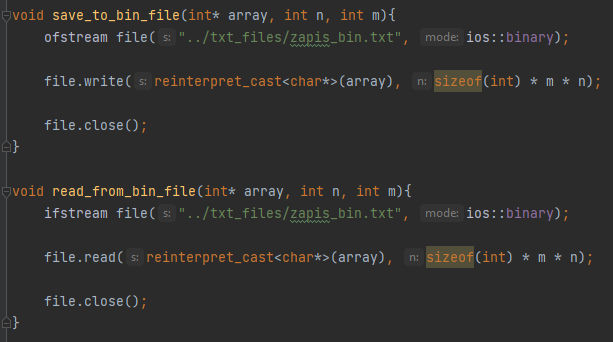
\includegraphics[width=0.5\linewidth]{pics/array_binfile}
		\caption{Zapis tablicy do pliku binarnego}
	\end{figure}
	
	\section{Zadanie 2 - Funkcje rekurencyjne.}
	\subsection{Matematyczne}
	Zadanie polegało na stworzeniu funkcji rekurencyjnych obliczających potęgę i silnię. Funkcja \textbf{potęga} rekurencyjnie tworzy iloczyn o długości wykładnika (np. $2^3 = 2 * 2 * 2$), zmniejszając go o jeden z każdym wywołaniem. Warunkiem wyjściowym z rekurencji jest osiągnięcie przez wykładnik wartości 1.
	\begin{itemize}
		\item Złożoność obliczeniowa: O(n),
		\item Złożoność pamięciowa: O(1).
	\end{itemize}
	\begin{figure}[h]
		\centering
		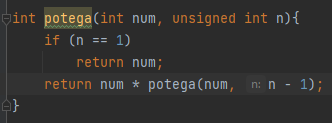
\includegraphics[width=0.7\linewidth, frame]{pics/pow_recursive}
		\caption{Rekurencyjna funkcja licząca potęgę.}
	\end{figure}
	Funkcja do obliczenia silni działa w ten sam sposób. Tworzy malejący iloczyn ciągu, aż do osiągnięcia jedynki  (np. $3! = 3 * 2 * 1$, gdzie 1 jest warunkiem wyjścia z rekurencji).
	\begin{itemize}
		\item Złożoność obliczeniowa: O(n),
		\item Złożoność pamięciowa: O(1).
	\end{itemize}
	\begin{figure}[h]
		\centering
		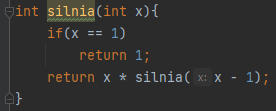
\includegraphics[width=0.7\linewidth, frame]{pics/sil_recursive}
		\caption{Rekurencyjna funkcja licząca średnią.}
	\end{figure}

	\newpage
	\subsection{Palindrom}
	Palindrom to słowo, które napisane od końca będzie takie samo. Funkcja działa poprzez odwoływanie się do zmiennej string po indeksach (jest traktowana jako tablica znaków). Kolejno sprawdzamy czy znaki są takie same, przesuwając "wskaźniki" bliżej środka wyrazu z każdą rekurencją. Jeśli w dowolnym momencie znaki będą inne, słowo nie jest palindromem i zwracany jest \textbf{fałsz}. Rekurencja kończy się, gdy lewy indeks będzie większy od prawego (wskaźniki "minęły" się, co oznacza że lewa i prawa część wyrazu została sprawdzona).
	\begin{itemize}
		\item Złożoność obliczeniowa: O(n),
		\item Złożoność pamięciowa: O(1).
	\end{itemize}
	\begin{figure}[h]
		\centering
		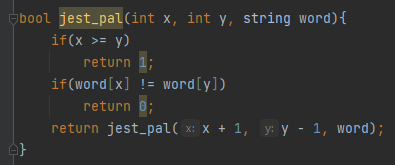
\includegraphics[width=0.7\linewidth, frame]{pics/palindrom_recursive}
		\caption{Rekurencyjna funkcja sprawdzająca czy słowo jest palindromem.}
	\end{figure}

	\newpage
	\subsection{Permutacje ciągu znaków}
	\subsubsection{Generacja palindromów}
	Funkcja przyjmuje tablice (rozmiar oparty na maksymalnej ilości wygenerowanych permutacji), do której zapisuje palindromy.
	\begin{itemize}
		\item Złożoność obliczeniowa: O(n!),
		\item Złożoność pamięciowa: O(1).
	\end{itemize}
	\begin{figure}[h]
		\centering
		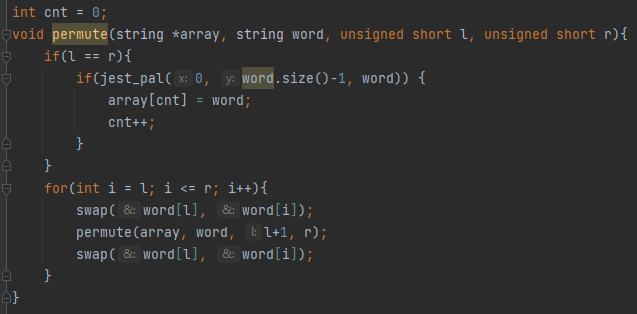
\includegraphics[width=0.55\linewidth]{pics/palindrom_gen}
		\caption{Funkcja generujące permutacje ciągu znaków i zapisująca palindromy.}
	\end{figure}
	
	\subsubsection{Usuwanie duplikatów}
	Funkcja zapisuje wyraz, a następnie sprawdza czy istnieją duplikaty (ignorując "puste" miejsca w tablicy). Jeśli powtórzenie wystąpi, to jest ono nadpisywane pustym stringiem.
	\begin{itemize}
		\item Złożoność obliczeniowa: O($n^2$),
		\item Złożoność pamięciowa: O(1).
	\end{itemize}
	\begin{figure}[h]
		\centering
		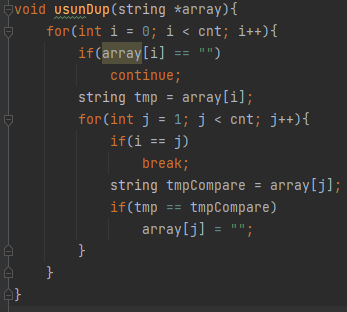
\includegraphics[width=0.4\linewidth]{pics/palindrom_usunDup}
		\caption{Funkcja usuwająca duplikowane palindromy.}
	\end{figure}
	
	\newpage
	\section{Struktury}
	\subsection{Węzeł}
	Każda z zaimplementowanych struktur opiera się na węzłach. Są to obiekty przechowujące wartość oraz wskaźnik na następny element.
	\begin{figure}[h]
		\centering
		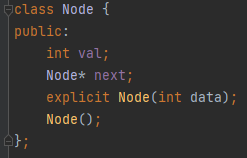
\includegraphics[width=0.5\linewidth]{pics/palindrom_recursive1}
		\caption{Struktura węzła.}
	\end{figure}
	
	\subsection{Lista jednokierunkowa}
	Lista jednokierunkowa jest prostą strukturą. Każdy element przechowuje wartość oraz wskaźnik na następny węzeł. Do listy odwołuje się przez "głowę" (czyli pierwszy element), a ostatni wskazuje na nic (nullptr).
	\begin{figure}[h]
		\centering
		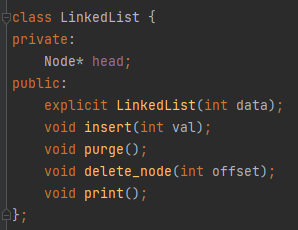
\includegraphics[width=0.45\linewidth, frame]{pics/linked_list}
		\caption{Klasa listy jednokierunkowej.}
	\end{figure}
	
	\subsubsection{Dodawanie}
	Metoda dzieli się na dwa przypadki. Dla pustej listy ustawiana jest nowa głowa. W innym przypadku tworzony jest tymczasowy wskaźnik, który przesuwany jest aż wskaże na ostatni węzeł, gdzie następnie jest dodawany nowy element.
	\newpage
	\begin{itemize}
		\item Złożoność obliczeniowa: O(n),
		\item Złożoność pamięciowa: O(1).
	\end{itemize}
	\begin{figure}[h]
		\centering
		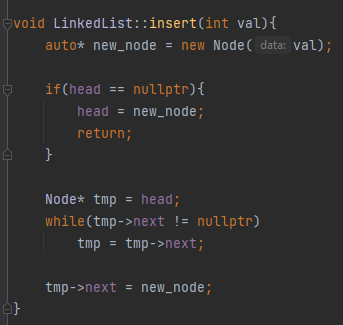
\includegraphics[width=0.45\linewidth]{pics/ll_insert}
		\caption{Metoda dodająca węzeł do listy.}
	\end{figure}
	
	\subsubsection{Usuwanie}
	Metoda sprawdza kilka sytuacji. Jeśli lista jest pusta wyświetla adekwatny komunikat. Jeśli istnieje jeden element, trzeba go usunąć i ustawić głowę na nullptr. Gdy usuwany jest pierwszy element trzeba przestawić głowę na nowy węzeł. W ostatnim przypadku usuwany jest podany węzeł oraz przepina się elementy.
	\begin{itemize}
		\item Złożoność obliczeniowa: O(n),
		\item Złożoność pamięciowa: O(1).
	\end{itemize}
	\begin{figure}[hh]
		\centering
		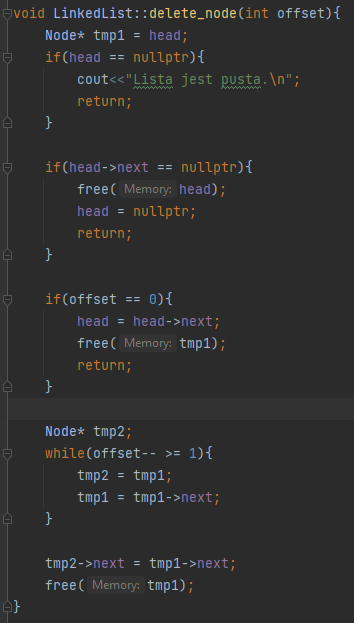
\includegraphics[width=0.5\linewidth]{pics/ll_delete}
		\caption{Metoda usuwająca węzeł}
	\end{figure}

	\newpage
	\subsubsection{Wyświetlanie}
	\label{ll_print}
	Dla pustej listy metoda wyświetla adekwatny komunikat. W innym przypadku metoda przechodzi przez wszystkie węzły, wyświetlając wartości, aż zacznie wskazywać na nullptr (pusty węzeł).
	\begin{itemize}
		\item Złożoność obliczeniowa: O(n),
		\item Złożoność pamięciowa: O(1).
	\end{itemize}
	\begin{figure}[h]
		\centering
		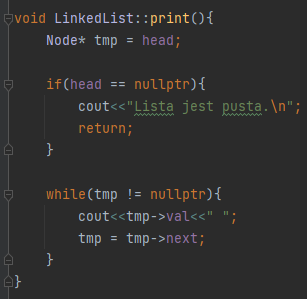
\includegraphics[width=0.4\linewidth]{pics/ll_print}
		\caption{Metoda wyświetlająca strukturę.}
	\end{figure}
	
	\newpage
	\subsubsection{Czyszczenie struktury}
	\label{ll_purge}
	Metoda zapisuję aktualną głowę listy, zmienia ją na następny element, następnie usuwa, powtarzając aż dojdzie do ostatniego węzła.
	\begin{itemize}
		\item Złożoność obliczeniowa: O(n),
		\item Złożoność pamięciowa: O(1).
	\end{itemize}
	\begin{figure}[h]
		\centering
		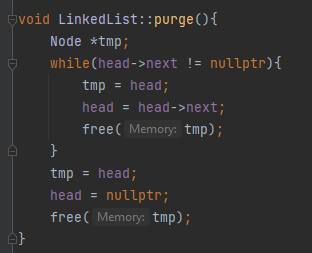
\includegraphics[width=0.4\linewidth]{pics/ll_purgfe}
		\caption{Metoda czyszcząca listę.}
	\end{figure}
	
	\subsection{Kolejka}
	Kolejka FIFO (first-in first-out) została zaimplementowana przez modyfikację listy jednokierunkowej. Jest uproszczeniem listy, ponieważ dla kolejki węzły zawsze dodajemy na końcu, a ściągamy z początku.
	
	\subsubsection{Dodawanie}
	Ponownie ostatni element nie jest zapamiętany, więc dla każdej operacji dodania metoda musi przejść przez wszystkie elementy, aby dodać nowy węzeł na końcu.
	\begin{itemize}
		\item Złożoność obliczeniowa: O(n),
		\item Złożoność pamięciowa: O(1).
	\end{itemize}
	\begin{figure}[h]
		\centering
		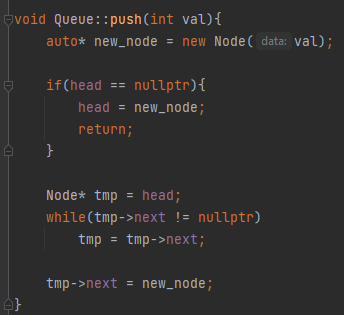
\includegraphics[width=0.5\linewidth]{pics/qu_insert}
		\caption{Metoda dodająca węzeł do kolejki.}
	\end{figure}

	\subsubsection{Usuwanie}
	Usuwany (i zwracany) jest pierwszy element, dlatego sama operacja jest bardzo szybka ponieważ do struktury odwołujemy się poprzez głowę (pierwszy element).
	\begin{itemize}
		\item Złożoność obliczeniowa: O(1),
		\item Złożoność pamięciowa: O(1).
	\end{itemize}
	\begin{figure}[h]
		\centering
		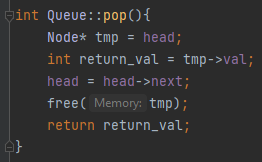
\includegraphics[width=0.5\linewidth]{pics/qu_pop}
		\caption{Metoda usuwająca element}
	\end{figure}
	
	\subsubsection{Wyświetlanie}
	\hyperref[ll_print]{Metoda wyświetlająca kolejkę jest identyczna jak dla listy jedno kierunkowej.}
	
	\subsubsection{Czysczenie kolejki}
	\hyperref[ll_purge]{Metoda czyszcząca kolejkę jest identyczna jak dla listy jedno kierunkowej.}
	
	\subsection{Dequeue}
	Dequeue jest strukturą podobną do kolejki, lecz możemy się odwołać do pierwszego elementu (head) i ostatniego (tail) oraz wykonywać na nich operacje dodawania i usuwania węzłów. Zadanie polegało na wykorzystaniu dequeue do sprawdzenia czy podany wyraz jest palindromem. Omówione zostaną tylko funkcję wykorzystane w tej metodzie (insert, shift, pop, isEmpty).
	\subsubsection{Węzeł}
	\begin{figure}[h]
		\centering
		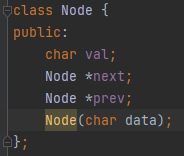
\includegraphics[width=0.4\linewidth]{pics/dequ_węzeł}
		\caption{Węzeł dla dequeue.}
	\end{figure}

	\subsubsection{Insert last}
	Dla pustej struktury węzeł jest ustawiony jednocześnie dla głowy i ogona. Jeśli węzły już istnieją wstawianie operacja odbywa się przez odwołanie do ogona. Dzięki temu wystarczy stworzyć węzeł, przepiąć wskaźniki i ustawić go jako nowy ogon.
	\begin{itemize}
		\item Złożoność obliczeniowa: O(1),
		\item Złożoność pamięciowa: O(1).
	\end{itemize}
	\begin{figure}[h]
		\centering
		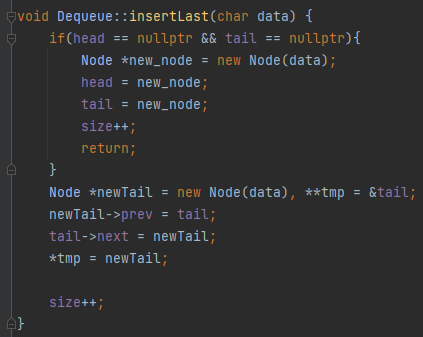
\includegraphics[width=0.5\linewidth, frame]{pics/dequ_insert}
		\caption{Metoda dodająca element na końcu dequeue.}
	\end{figure}
	
	\newpage
	\subsubsection{Shift, Pop}
	Obydwie metody usuwające działają na tej samej zasadzie poprzez operacje na odpowiednim końcu struktury. Operacja polega na przepięciu krańcowego węzła na nowy i usunięcie starego węzła. Na końcu zwracana jest wartość usuniętego elementu.
	\begin{figure}[h]
		\begin{subfigure}{0.45\linewidth}
			\centering
			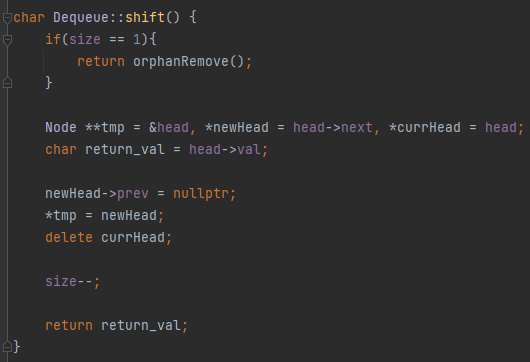
\includegraphics[width=1\linewidth]{pics/dequ_shift}
			\caption{Usuwanie elementów z początku dequeue.}
		\end{subfigure}
	\hfill
		\begin{subfigure}{0.45\linewidth}
			\centering
			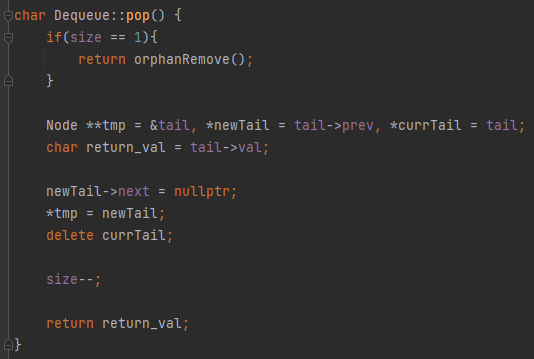
\includegraphics[width=1\linewidth]{pics/dequ_pop}
			\caption{Usuwanie elementów z końca dequeue.}
		\end{subfigure}
	\caption{Metody usuwania elementów.}
	\end{figure}
	
	\newpage
	\subsubsection{isEmpty}
	Żeby sprawdzić czy dequeue jest puste odwołujemy się do wskaźników na głowę i ogon. Przy pustej strukturze pierwszy element jest ustawiany na dwa wskaźniki, a dla usuwania ostatniego elementu (orphanRemove) metoda dba aby ustawić wskaźniki na nullptr.
	\begin{figure}[h]
		\centering
		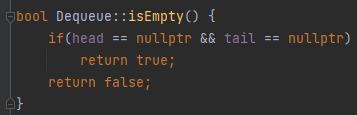
\includegraphics[width=0.6\linewidth, frame]{pics/dequ_isEmpty}
		\caption{Metoda sprawdzający czy dequeue nie zawiera węzłów.}
	\end{figure}
	
	
\end{document}
